\documentclass[dvipdfmx]{jarticle}
\pagestyle{empty}
\usepackage{tikz}
\usetikzlibrary{calc,shapes}
\begin{document}
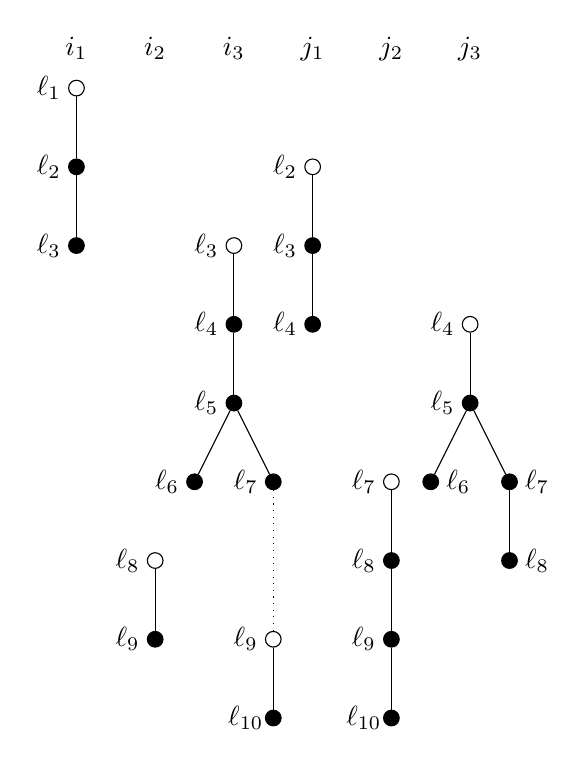
\begin{tikzpicture}
\node at (0,0) {$i_1$};
\node at (1,0) {$i_2$};
\node at (2,0) {$i_3$};
\node at (3,0) {$j_1$};
\node at (4,0) {$j_2$};
\node at (5,0) {$j_3$};
\node[draw,circle,inner sep=2pt] (I11) at (0,-0.5) {};
\node at ($(I11)+(-0.35,0)$) {$\ell_1$};
\node[draw,circle,inner sep=2pt,fill=black] (I12) at (0,-1.5) {};
\node at ($(I12)+(-0.35,0)$) {$\ell_2$};
\node[draw,circle,inner sep=2pt,fill=black] (I13) at (0,-2.5) {};
\node at ($(I13)+(-0.35,0)$) {$\ell_3$};
\path[-] (I11) edge (I12) (I12) edge (I13);
% i2
\node[draw,circle,inner sep=2pt] (I21) at (1,-6.5) {};
\node at ($(I21)+(-0.35,0)$) {$\ell_8$};
\node[draw,circle,inner sep=2pt,fill=black] (I22) at (1,-7.5) {};
\node at ($(I22)+(-0.35,0)$) {$\ell_9$};
\path[-] (I21) edge (I22);
% i3
\node[draw,circle,inner sep=2pt] (I31) at (2,-2.5) {};
\node at ($(I31)+(-0.35,0)$) {$\ell_3$};
\node[draw,circle,inner sep=2pt,fill=black] (I32) at (2,-3.5) {};
\node at ($(I32)+(-0.35,0)$) {$\ell_4$};
\node[draw,circle,inner sep=2pt,fill=black] (I33) at (2,-4.5) {};
\node at ($(I33)+(-0.35,0)$) {$\ell_5$};
\node[draw,circle,inner sep=2pt,fill=black] (I34) at (1.5,-5.5) {};
\node at ($(I34)+(-0.35,0)$) {$\ell_6$};
\node[draw,circle,inner sep=2pt,fill=black] (I35) at (2.5,-5.5) {};
\node at ($(I35)+(-0.35,0)$) {$\ell_7$};
\node[draw,circle,inner sep=2pt] (I36) at (2.5,-7.5) {};
\node at ($(I36)+(-0.35,0)$) {$\ell_9$};
\node[draw,circle,inner sep=2pt,fill=black] (I37) at (2.5,-8.5) {};
\node at ($(I37)+(-0.35,0)$) {$\ell_{10}$};
\path[-] (I31) edge (I32) (I32) edge (I33) (I33) edge (I34) (I33) edge (I35) (I36) edge (I37);
\path[style=dotted] (I35) edge (I36);
% j1
\node[draw,circle,inner sep=2pt] (J11) at (3,-1.5) {};
\node at ($(J11)+(-0.35,0)$) {$\ell_2$};
\node[draw,circle,inner sep=2pt,fill=black] (J12) at (3,-2.5) {};
\node at ($(J12)+(-0.35,0)$) {$\ell_3$};
\node[draw,circle,inner sep=2pt,fill=black] (J13) at (3,-3.5) {};
\node at ($(J13)+(-0.35,0)$) {$\ell_4$};
\path[-] (J11) edge (J12) (J12) edge (J13);
% j2
\node[draw,circle,inner sep=2pt] (J21) at (4,-5.5) {};
\node at ($(J21)+(-0.35,0)$) {$\ell_7$};
\node[draw,circle,inner sep=2pt,fill=black] (J22) at (4,-6.5) {};
\node at ($(J22)+(-0.35,0)$) {$\ell_8$};
\node[draw,circle,inner sep=2pt,fill=black] (J23) at (4,-7.5) {};
\node at ($(J23)+(-0.35,0)$) {$\ell_9$};
\node[draw,circle,inner sep=2pt,fill=black] (J24) at (4,-8.5) {};
\node at ($(J24)+(-0.35,0)$) {$\ell_{10}$};
\path[-] (J21) edge (J22) (J22) edge (J23) (J23) edge (J24);
% j3
\node[draw,circle,inner sep=2pt] (J31) at (5,-3.5) {};
\node at ($(J31)+(-0.35,0)$) {$\ell_4$};
\node[draw,circle,inner sep=2pt,fill=black] (J32) at (5,-4.5) {};
\node at ($(J32)+(-0.35,0)$) {$\ell_5$};
\node[draw,circle,inner sep=2pt,fill=black] (J33) at (4.5,-5.5) {};
\node at ($(J33)+(0.35,0)$) {$\ell_6$};
\node[draw,circle,inner sep=2pt,fill=black] (J34) at (5.5,-5.5) {};
\node at ($(J34)+(0.35,0)$) {$\ell_7$};
\node[draw,circle,inner sep=2pt,fill=black] (J35) at (5.5,-6.5) {};
\node at ($(J35)+(0.35,0)$) {$\ell_8$};
\path[-] (J31) edge (J32) (J32) edge (J33) (J32) edge (J34) (J34) edge (J35);
\end{tikzpicture}
\end{document}